\chapter{Hardware Design} \label{chap:HardwareDesign}

\section{Version}
\begin{table}[h]
	\centering
	\begin{tabularx}{\textwidth - 2cm}{|l|l| l|X|}
	\hline
	Dato	& Version	& Initialer & Ændring. \\ \hline
	01. december & 1 & LS	& Første version af dokumentet. \\ \hline
	02. december & 2 & HBJ	& Diverse design ændringer. \\ \hline
	15. december & 3 & LS & Små rettelser. Endelige version. \\ \hline
	\end{tabularx} 
\end{table}

\section{Blokopdeling}

Systemets hardware er opdelt i en transmitter- og to receiverdele. 
De underblokke der optræder flere steder i systemet er ens, og beskrives derfor kun én gang. For samtlige diagrammer gælder, at de resterende ikke anvendte inputs på IC'er, der ikke er vist, er koblet til stel.

\begin{figure}[h]
	\centering
	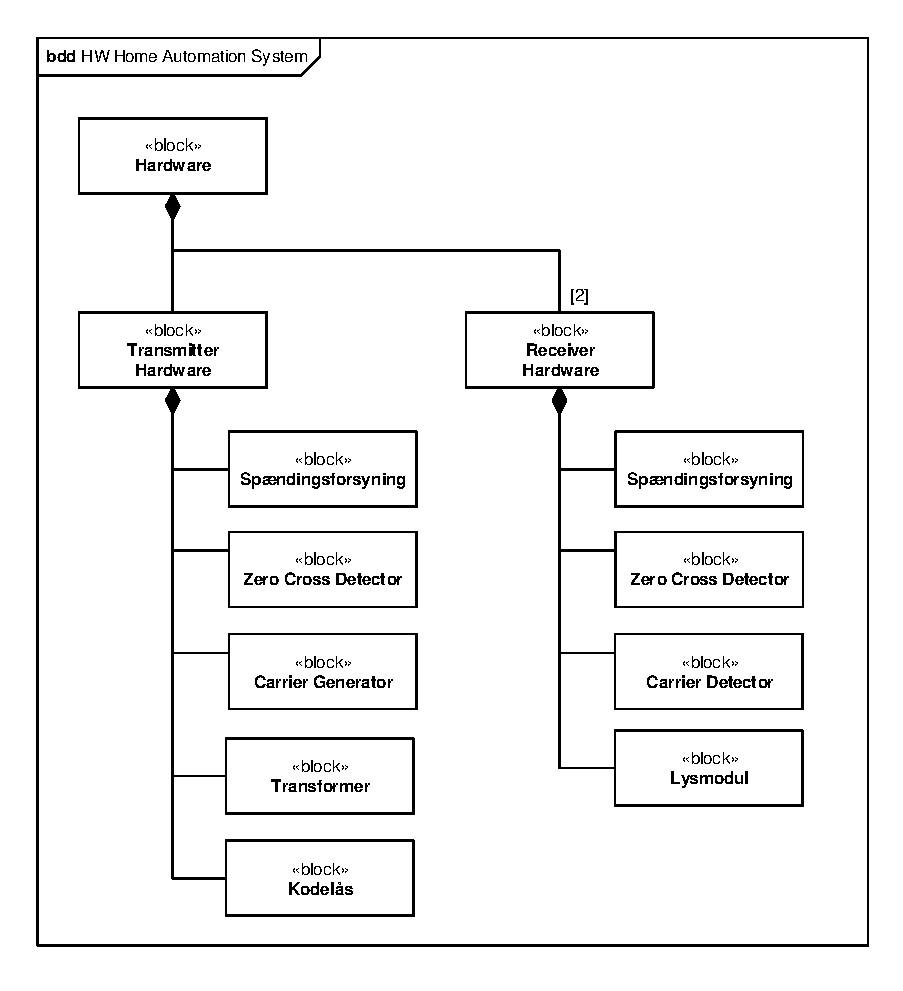
\includegraphics[scale=0.75, trim=10 10 10 10, clip=true]{../HardwareDesign/Diagrammer/BDD_HW.pdf}
	\caption{BDD-diagram over hardware}
	\label{fig:HWBDD}
\end{figure}

\section{Transmitter}

\subsection{18V AC Transformer}
Transformeren ($8610AC$)\cite{lib:Adaptor} transformerer $230V AC$ til $18V AC$, således at det er muligt at simulere et elnet.

\subsection{Spændingsforsyning (Morten)}
Systemet skal forsynes med en $5V$ og en $-5V$ spænding. Spændingsforsyningen forsynes med 12V DC fra en ekstern spændingskilde. Der er anvendt en positiv fastspændingsregulator ($LM7805$)\cite{lib:LM7805} og en spændings-inverter($ICL7660$)\cite{lib:IC7660}, og de er opsat jf. standardapplikationen i deres respektive datablade.
$500 mA$ er den den mindste tilgængelige sikring, derfor er denne valgt, da der ikke forventes en samlet strøm, der er større end dette i nogen af de tre spændingsforsyninger (transmitter og to receivere). Dette giver et forholdsvis stort spændingsfald over spændingsregulatoren, hvorfor den monteres med køleplade, for at undgå overophedning. 
Kredsløbets design er vist i Figur \ref{fig:Stromforsyning}.
\begin{figure}[h]
	\centering
	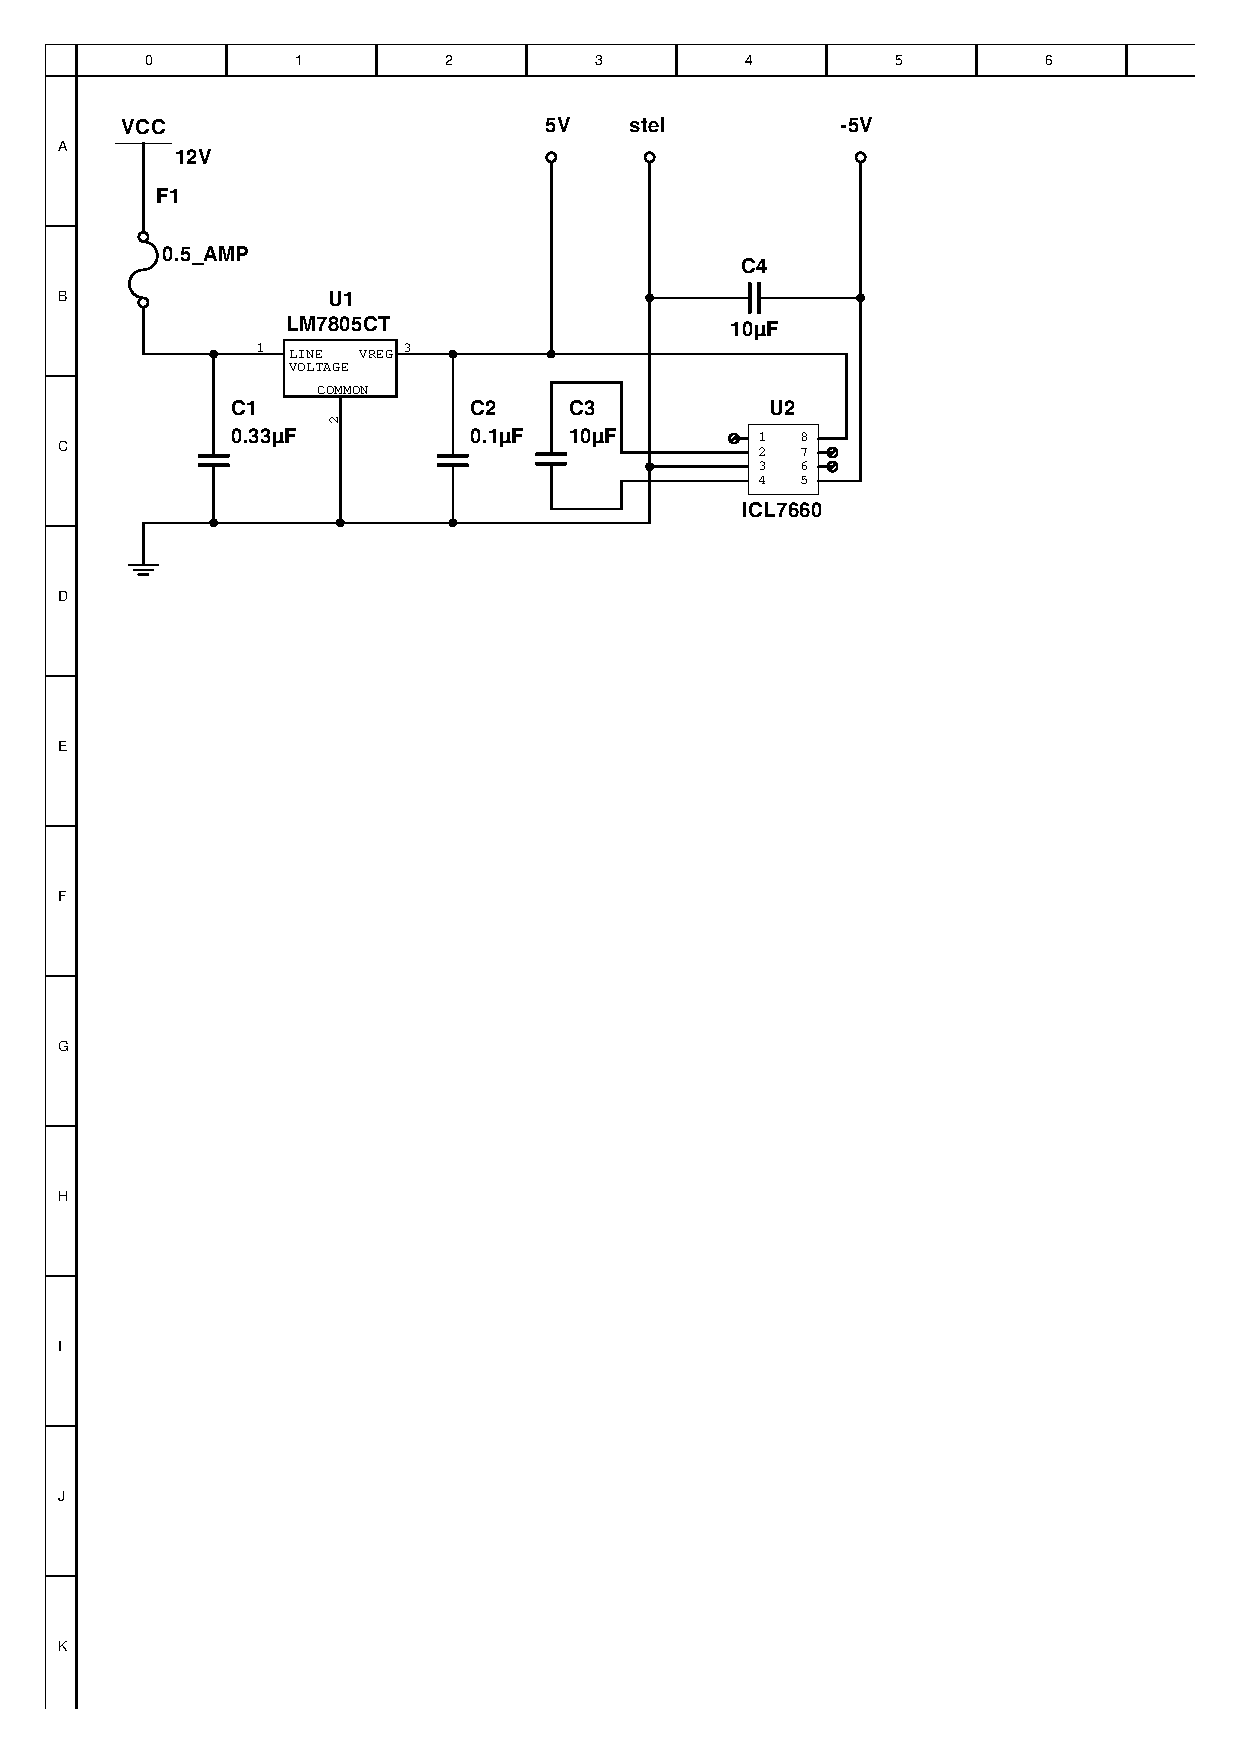
\includegraphics[scale=1,trim=50 555 150 50, clip=true]{../HardwareDesign/Diagrammer/Stroemforsyning.pdf}
	\caption{Spændingsforsyning}
	\label{fig:Stromforsyning}
\end{figure}

\subsection{Kodelås (Lasse og Henrik)}
Kodelåsen sender et \textit{HIGH} signal ud på DE2-boardet's ben JP1-10 ($GPIO{\_}0[9]$), når der ikke er indtastet tre rigtige koder. Så snart koderne er indtastet korrekt, vil dette signal skifte fra \textit{HIGH} til \textit{LOW}. Hvis der indtastes forkert kode 3 gange, vil kodelåsen gå i en permanent låsetilstand, som kræver manuel reset. Desuden er der fælles ground fra JP1-12 ($Ground$).
Denne blok er lavet under en øvelse i faget Digital System Design, og er derfor ikke forklaret yderligere under dette afsnit.

\subsection{Zerocross Detector (Morten og Philip)}
Zerocross detectoren (Figur \ref{fig:ZeroCrossDetect}) har til formål at toggle ZeroCrossDetect signalet, når der registreres en nul-gennemgang på $18VAC$ - $50Hz$ nettet. Kredsløbet består af et højpasfilter, to dioder $(1N4148)$\cite{lib:1N4148}, der har til formål at begrænse spændingen til $0.7V$ og en operationsforstærker $(TS912)$\cite{lib:TS912}. Operationsforstærkeren giver et output alt efter om inputtet på plus-benet er højere eller lavere end inputtet på minus-benet, der er koblet til stel. 

Da der vil være risiko for prel i nul-gennemgangene på udgangen af operationsforstærkeren, opbygges kredsløbet som i Figur \ref{fig:ZeroCrossDetect}, således at der fremkommer en hysterese. Tærskelværdierne for hysteresen sættes til $\pm 100mV$ således at den samlede hysterese bliver $200mV$. På baggrund af dette kan værdierne for $R_{2}$ og $R_{3}$ bestemmes.

Beregningerne er fortaget for det tilfælde, lige før en nedadgående nul-gennemgang finder sted.

Spændingsfaldet over $R_{2}$ skal være $V_{R_{2}}=100mV$

$R_{2}$ sættes til $1k\Omega$

Når operationsforstærkeren skal gå fra høj til lav er spændingen på udgangen $V_{out}=5V$.

\begin{displaymath}
V_{R_{2}}=V_{out} \cdot \dfrac{R_{2}}{R_{2}+R_{3}} \Rightarrow
R_{3}=\dfrac{R_{2} \cdot V_{out}}{V_{R_{2}}}-R_{2}=
\dfrac{1k\Omega \cdot 5V}{100mV}-1k\Omega=49k\Omega\approx47k\Omega
\end{displaymath}

For at undgå negativ spænding på ZeroCrossDetect signalet, er der placeret en diode ($D_{3}$), som forhindrer dette. Der er et mindre spændingfald over dioden, men dette har ingen betydning. Derudover er der forbundet en pull-down modstand ($R_{15}$) efter dioden, for at sikre at signalet ligger stabilt på $0V$, når operationsforstærkeren leverer negativ spænding.
\begin{figure}[h]
	\centering
	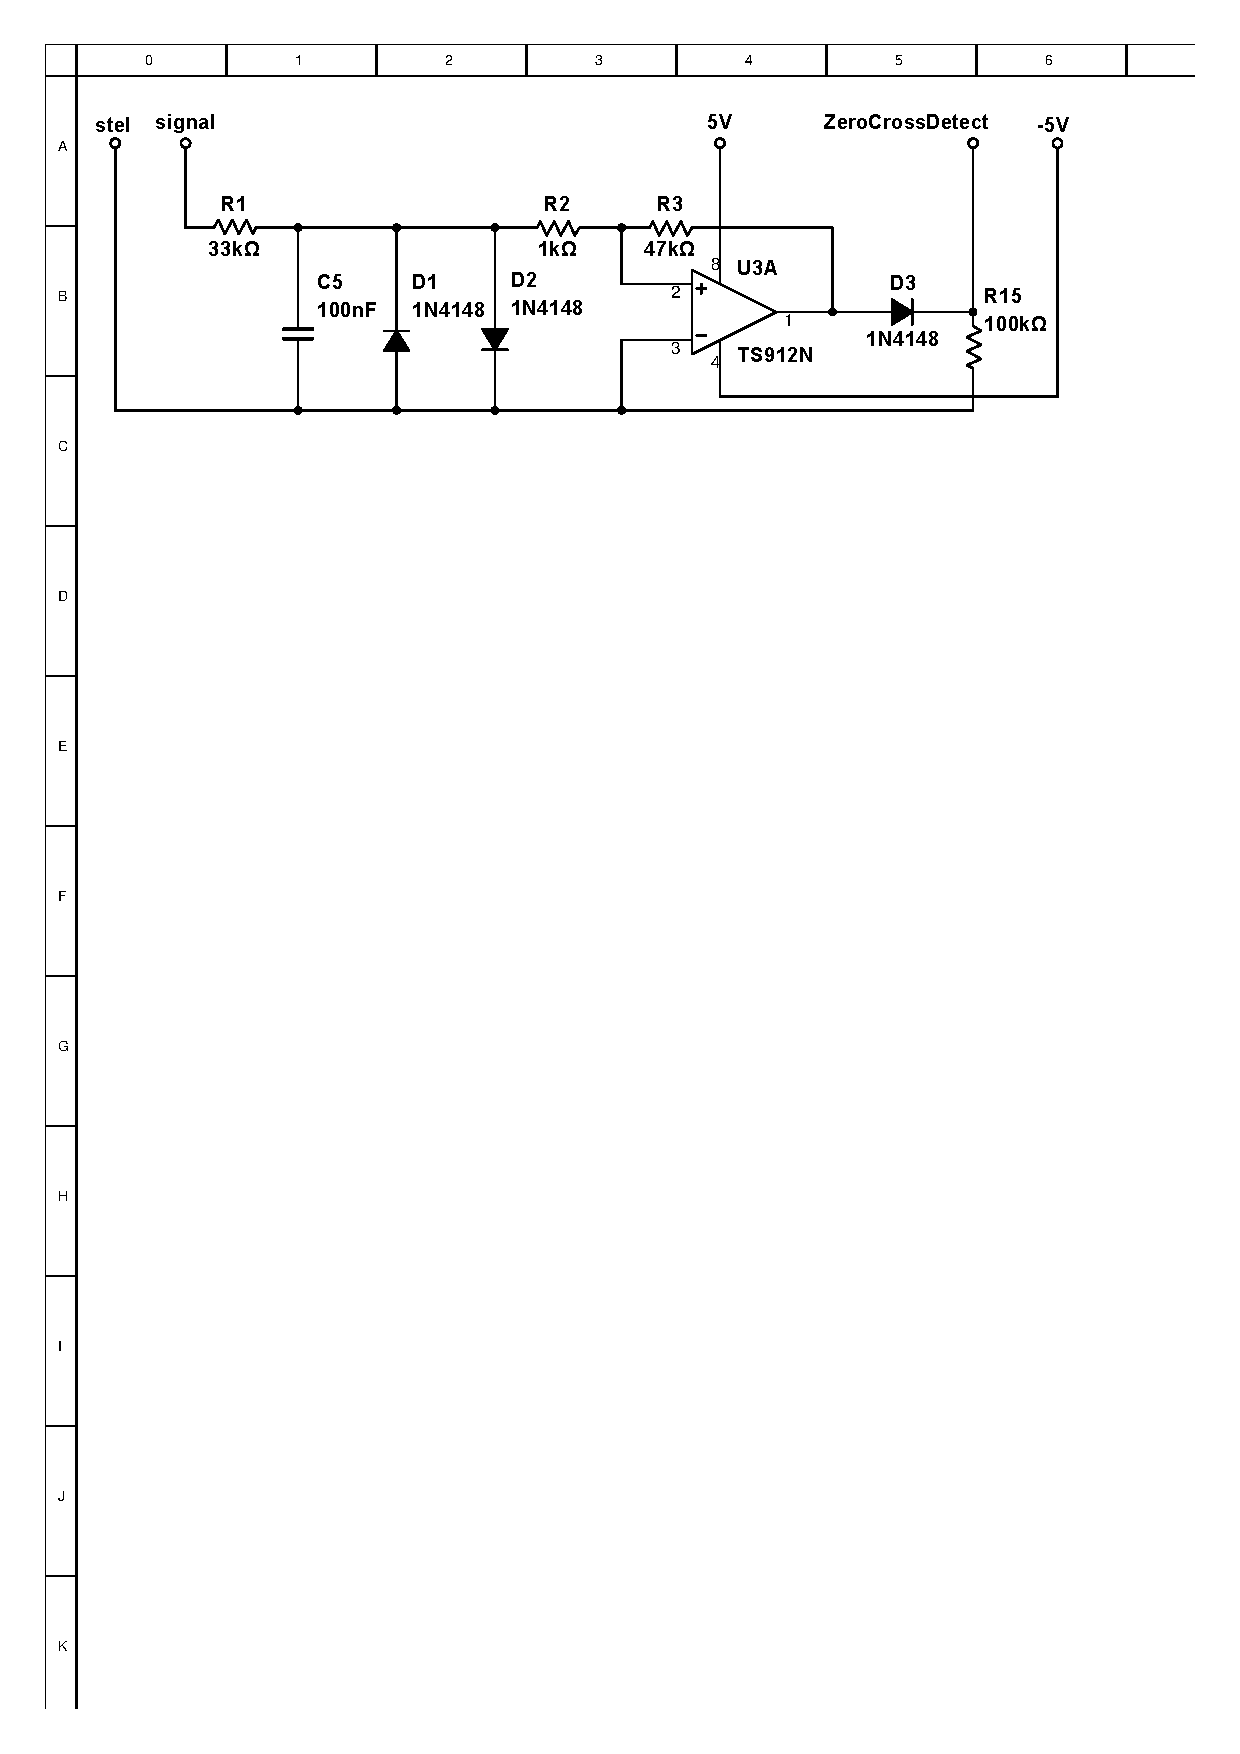
\includegraphics[scale=1, trim=45 635 80 50, clip=true]{../HardwareDesign/Diagrammer/ZeroCrossDetector.pdf}
	\caption{Zerocross detector}
	\label{fig:ZeroCrossDetect}
\end{figure}

For lavpasfiltret $R_{1}$ og $C_{5}$ fås overføringsfunktionen:

\begin{displaymath}
T_{v}(s) \approx \dfrac{\tfrac{1}{C_{5} \cdot s}}{\tfrac{1}{C_{5} \cdot s} + R_{1}} =
\dfrac{\tfrac{1}{R_{1}C_{5}}}{s+\tfrac{1}{R_{1}C_{5}}}
\end{displaymath}

For lavpasfiltret sættes knækfrekvensen til:

\begin{displaymath}
\omega_{c_{1}}=2\cdot \pi \cdot 50Hz = 100\pi rad/s
\end{displaymath}
Det vides at knækfrekvensen $\omega_{c_{1}}$ svarer til leddet $\dfrac{1}{R_{1}C_{5}}$


$C_{5}$ sættes til at være $100nF$, derfor:

\begin{displaymath}
R_{1}= \dfrac{1}{\omega_{c_{1}}\cdot C_{5}} =
\dfrac{1}{100\pi s^{-1} \cdot 100\cdot 10^{-9}F} =
31.8k\Omega \approx 33k\Omega
\end{displaymath}

Der opstilles et bodeplot med asymptotiske linjer for lavpasfiltret, Figur \ref{fig:BodePlotLPF}.

Gain i knækfrekvensen $\omega_{c_{1}}$ er $-3dB$, men det har ikke nogen funktionel betydning.

\begin{figure}[h]
	\centering
	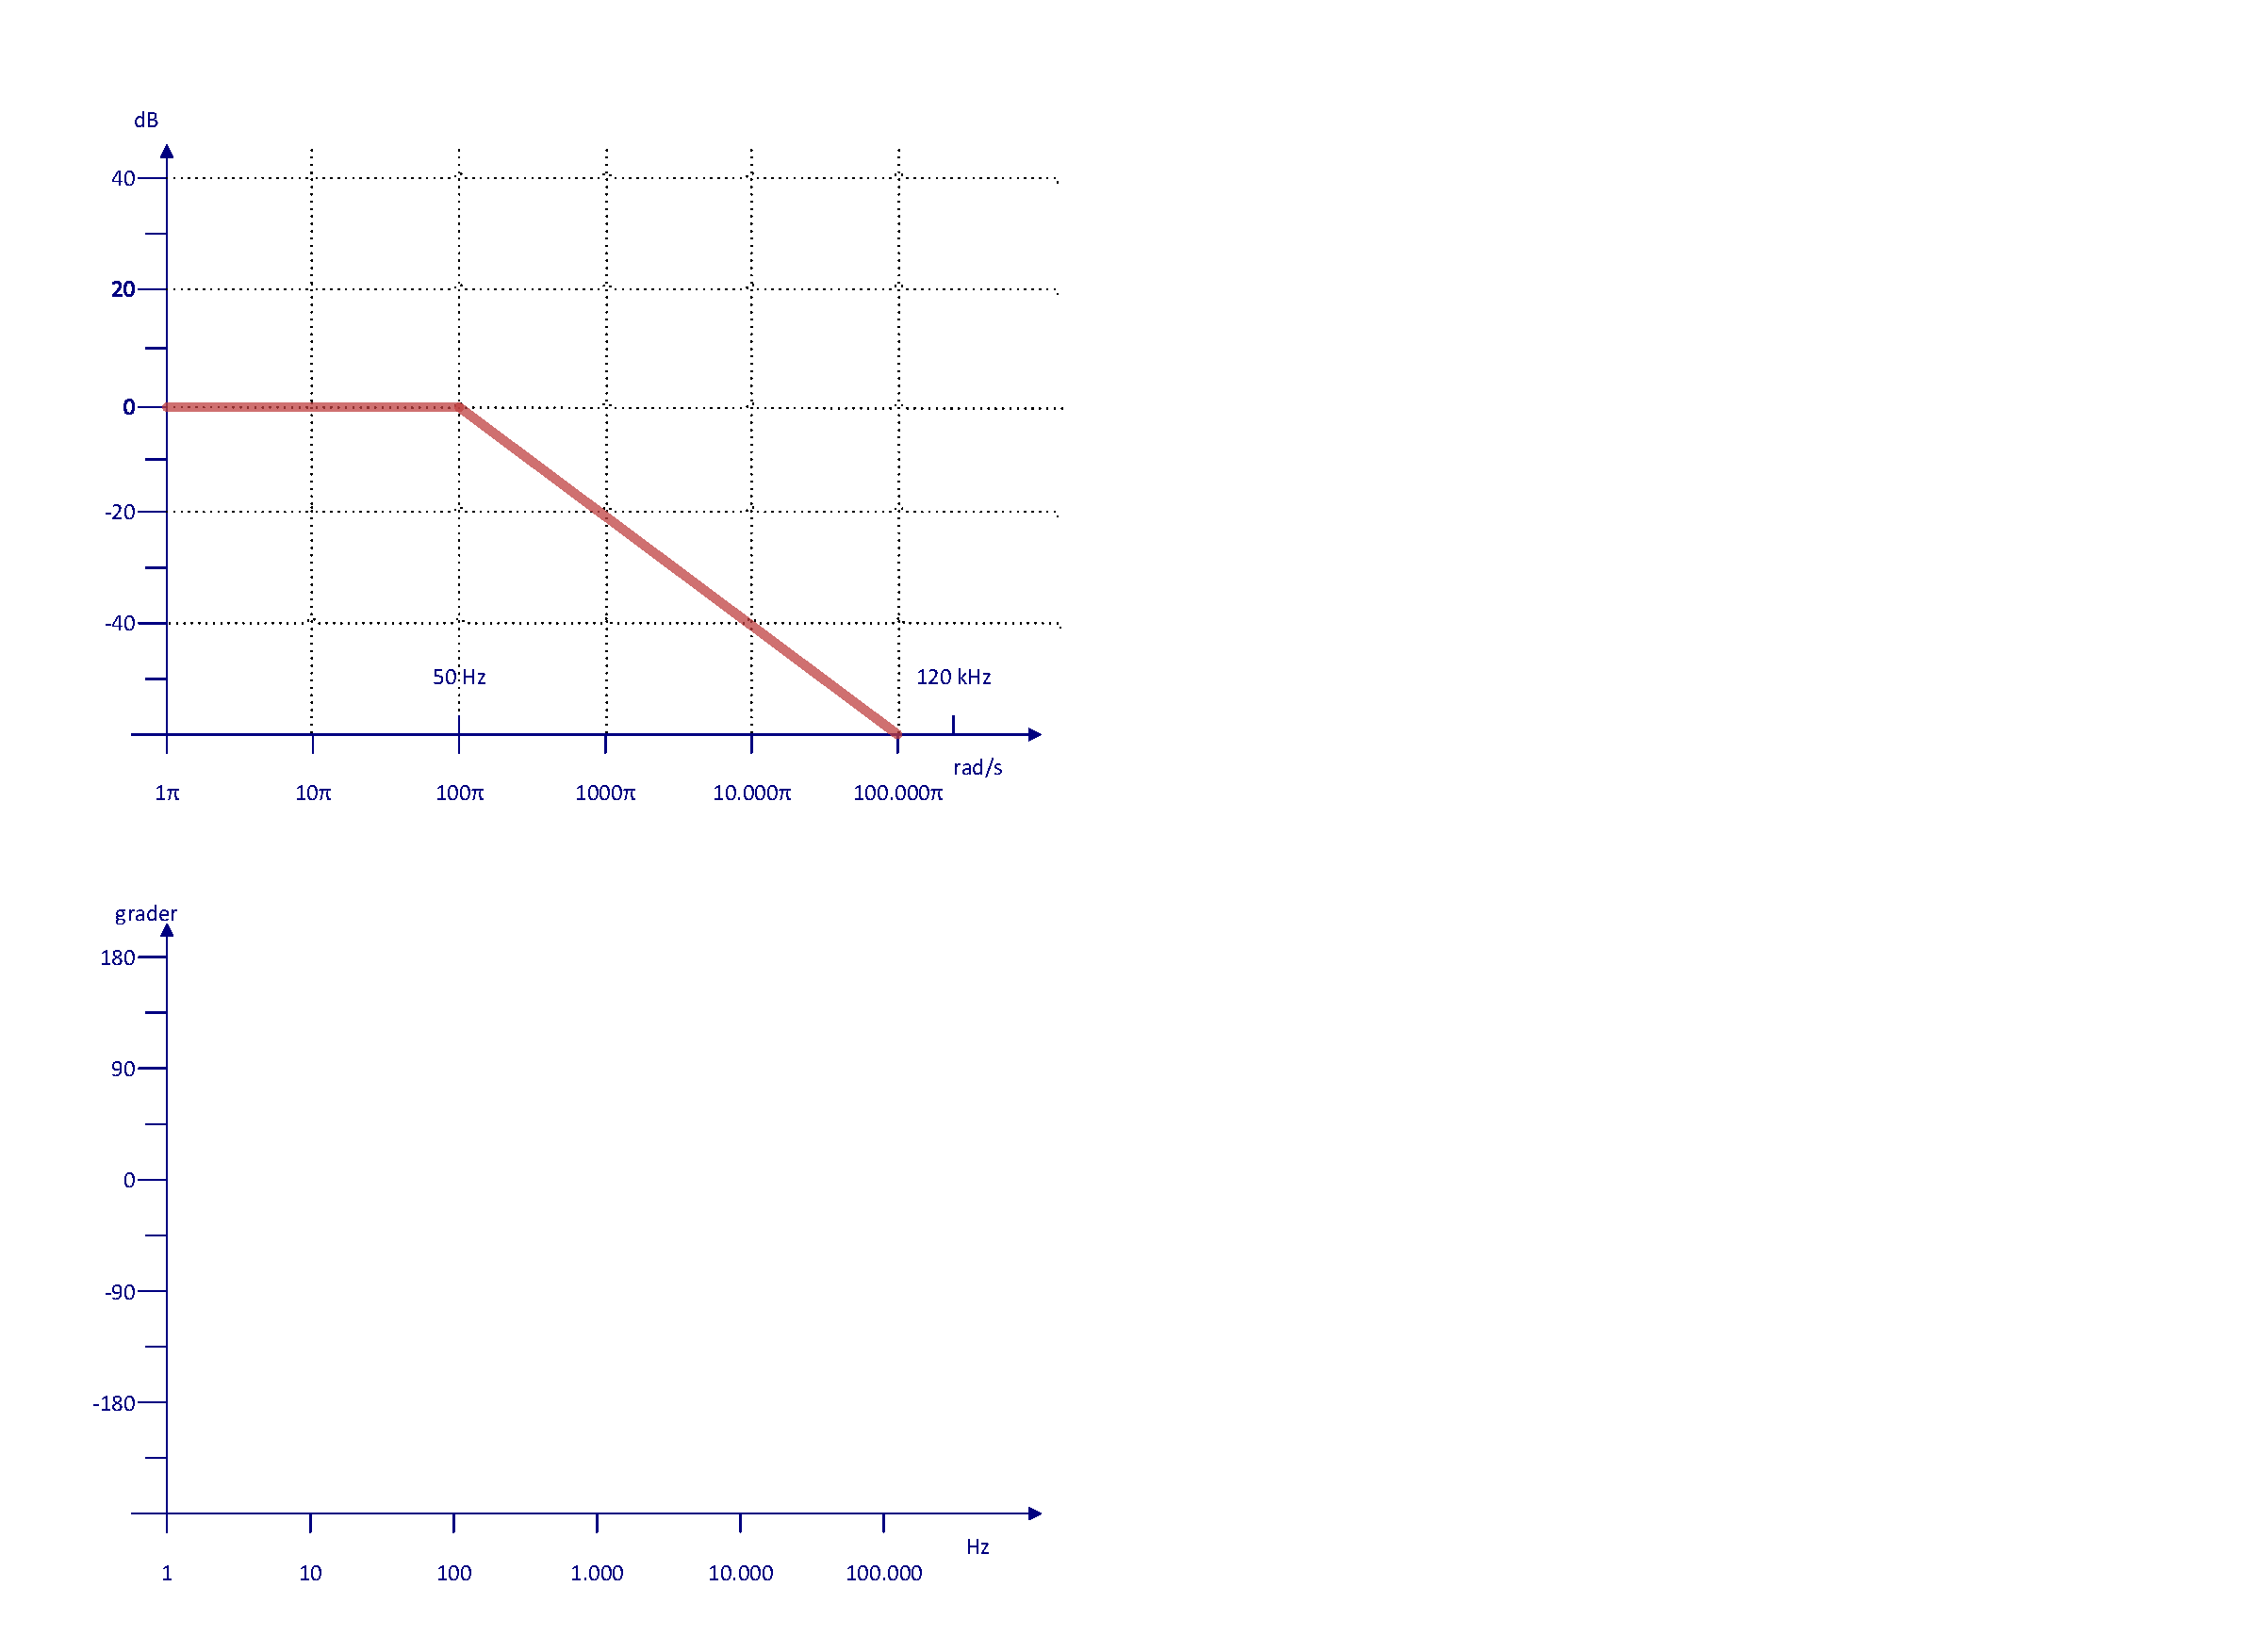
\includegraphics[scale=0.6, trim=50 430 590 50, clip=true]{../HardwareDesign/Diagrammer/BodePlotLPF.pdf}
	\caption{Bodeplot med asymptotiske linjer for lavpasfilter}
	\label{fig:BodePlotLPF}
\end{figure}

\newpage

\subsection{Carrier Generator (Philip og Lasse)} \label{subSecCarrierGen}

For at transmitteren uforstyrret kan sende et $120kHz$ signal på el-nettet, designes et kredsløb, der skal forhindre påvirkning fra $18VAC$ - $ 50Hz$ nettet på transmitter-hardwaren. Dette gøres vha. et  højpasfilter, samt et transistor-kredsløb som vist i Figur \ref{fig:CarrierGenDesign}.

\begin{figure}[h]
	\centering
	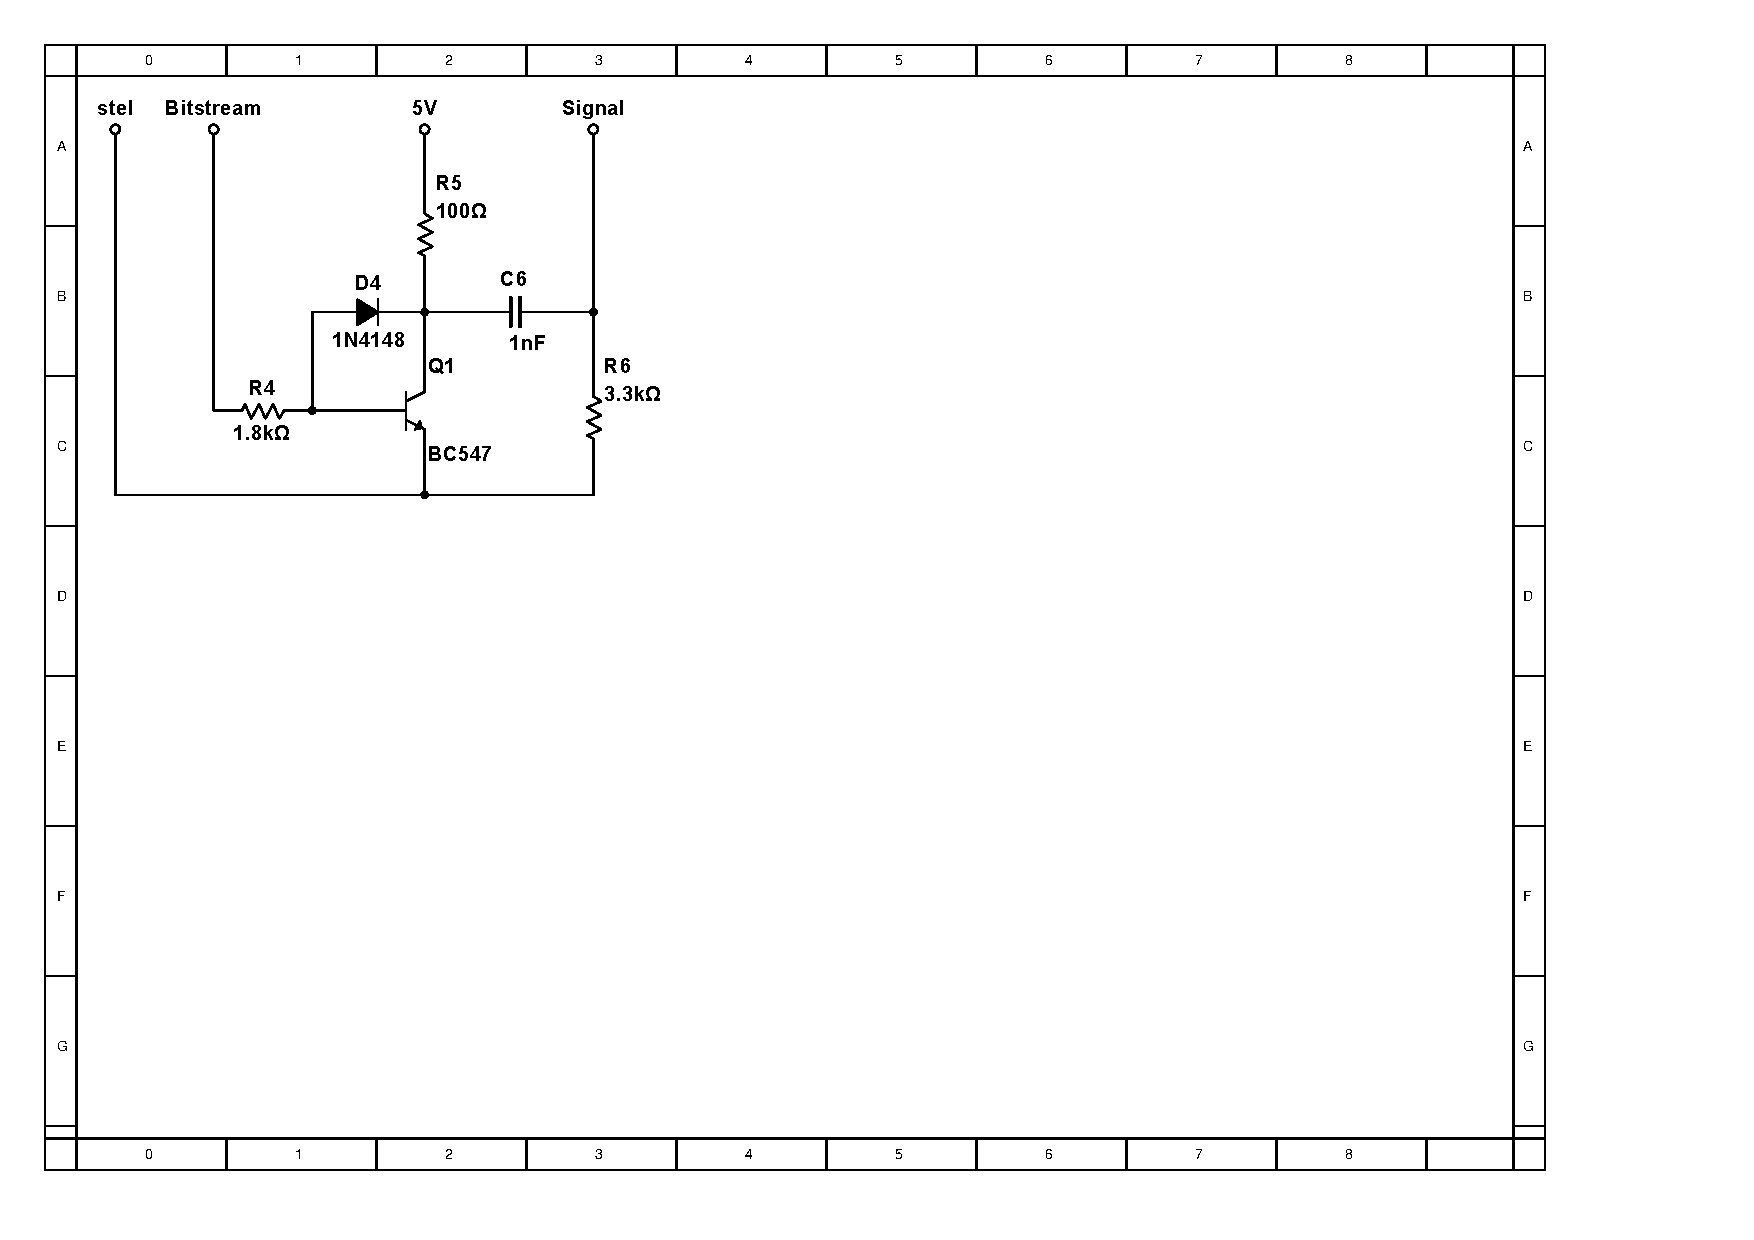
\includegraphics[scale=0.8, trim=45 355 525 45, clip=true]{../HardwareDesign/Diagrammer/CarrierGenerator.pdf}
	\caption{Carrier generator}
	\label{fig:CarrierGenDesign}
\end{figure}

Komponenternes værdier er udregnet på følgende måde:

For at transistoren $(BC547)$\cite{lib:BC547} er i mætning, skal basestrømmen $I_{b}$ være max. $20$ gange lavere end kollektorstrømmen $I_{c}$, dvs. transistorens $\beta\text{-værdi} \leq 20$. Der vælges en kollektor modstand $R_{5}=100\Omega$, derefter kan vælges en basemodstand der max er 20 gange større end kollektormodstanden, for at ovenstående krav er overholdt. Grunden til dette er at \textit{Bitstream} har samme spænding som de $5V$ på spændingsforsyningen når den er HIGH.

Der vælges derfor en basemodstand $R_{4}=1.8k\Omega$, hvilket gør at der kun bliver trukket $\tfrac{5V}{1.8 \cdot 10^{3}\Omega}=2.8mA$ fra \textit{Bitstream}. Basestrømmen bliver trukket fra STK500, og det ønskes derfor ikke, at der bliver trukket en særlig stor strøm derfra. Der er placeret en diode $(D4)$ mellem transistorens base- og kollektor ben, med spærreretning mod kollektoren, for at hjælpe tranistoren med at aflade positiv opladning. Af samme årsag er transistoren $BC547$ valgt, da denne har et mindre storage delay.

\subsubsection{Højpasfilter}

For højpasfilteret på Figur \ref{fig:CarrierGenDesign}, kan følgende overføringsfunktion opstilles:\\\\
\begin{displaymath}
T_{v}(s)\approx
\dfrac{R_{6}}{\tfrac{1}{C_{6}\cdot s}+R_{6}}=
\dfrac{R_{6} \cdot s}{\tfrac{1}{C_{6}} + R_{6} }=
\dfrac{s}{ \tfrac{1}{R_{6} \cdot C_{6}}+s }=
\dfrac{\tfrac{1}{R_{6}\cdot C_{6}}}{\tfrac{1}{R_{6}\cdot C_{6}}+s} \cdot \dfrac{s}{\tfrac{1}{R_{6}\cdot C_{6}}}
\end{displaymath}

Frekvensen der skal transmitteres igennem filteret er:

\begin{displaymath}
\omega_{120k} = 120kHz\cdot 2 \pi = 240000 \pi rad/s = 7.54\cdot 10^{5} rad/s
\end{displaymath}

Frekvensen fra transformeren, som \textit{ikke} skal kunne passere igennem filteret, er:
\begin{displaymath}
\omega_{50} = 50Hz\cdot 2 \pi = 100 \pi rad/s = 314.16 rad/s
\end{displaymath}

Med denne viden fastsættes knækfrekvensen $\omega_{c_{2}}$ til:

\begin{displaymath}
\omega_{c_{2}}= 2\pi \cdot 50kHz = 100\cdot 10^{3}\pi rad/s
\end{displaymath}

Derved bliver alle frekvenser under $100\cdot 10^{3}\pi$ $rad/s$ dæmpet, og den endelige overføringsfunktion bliver således:

\begin{figure}[h]
	\centering
	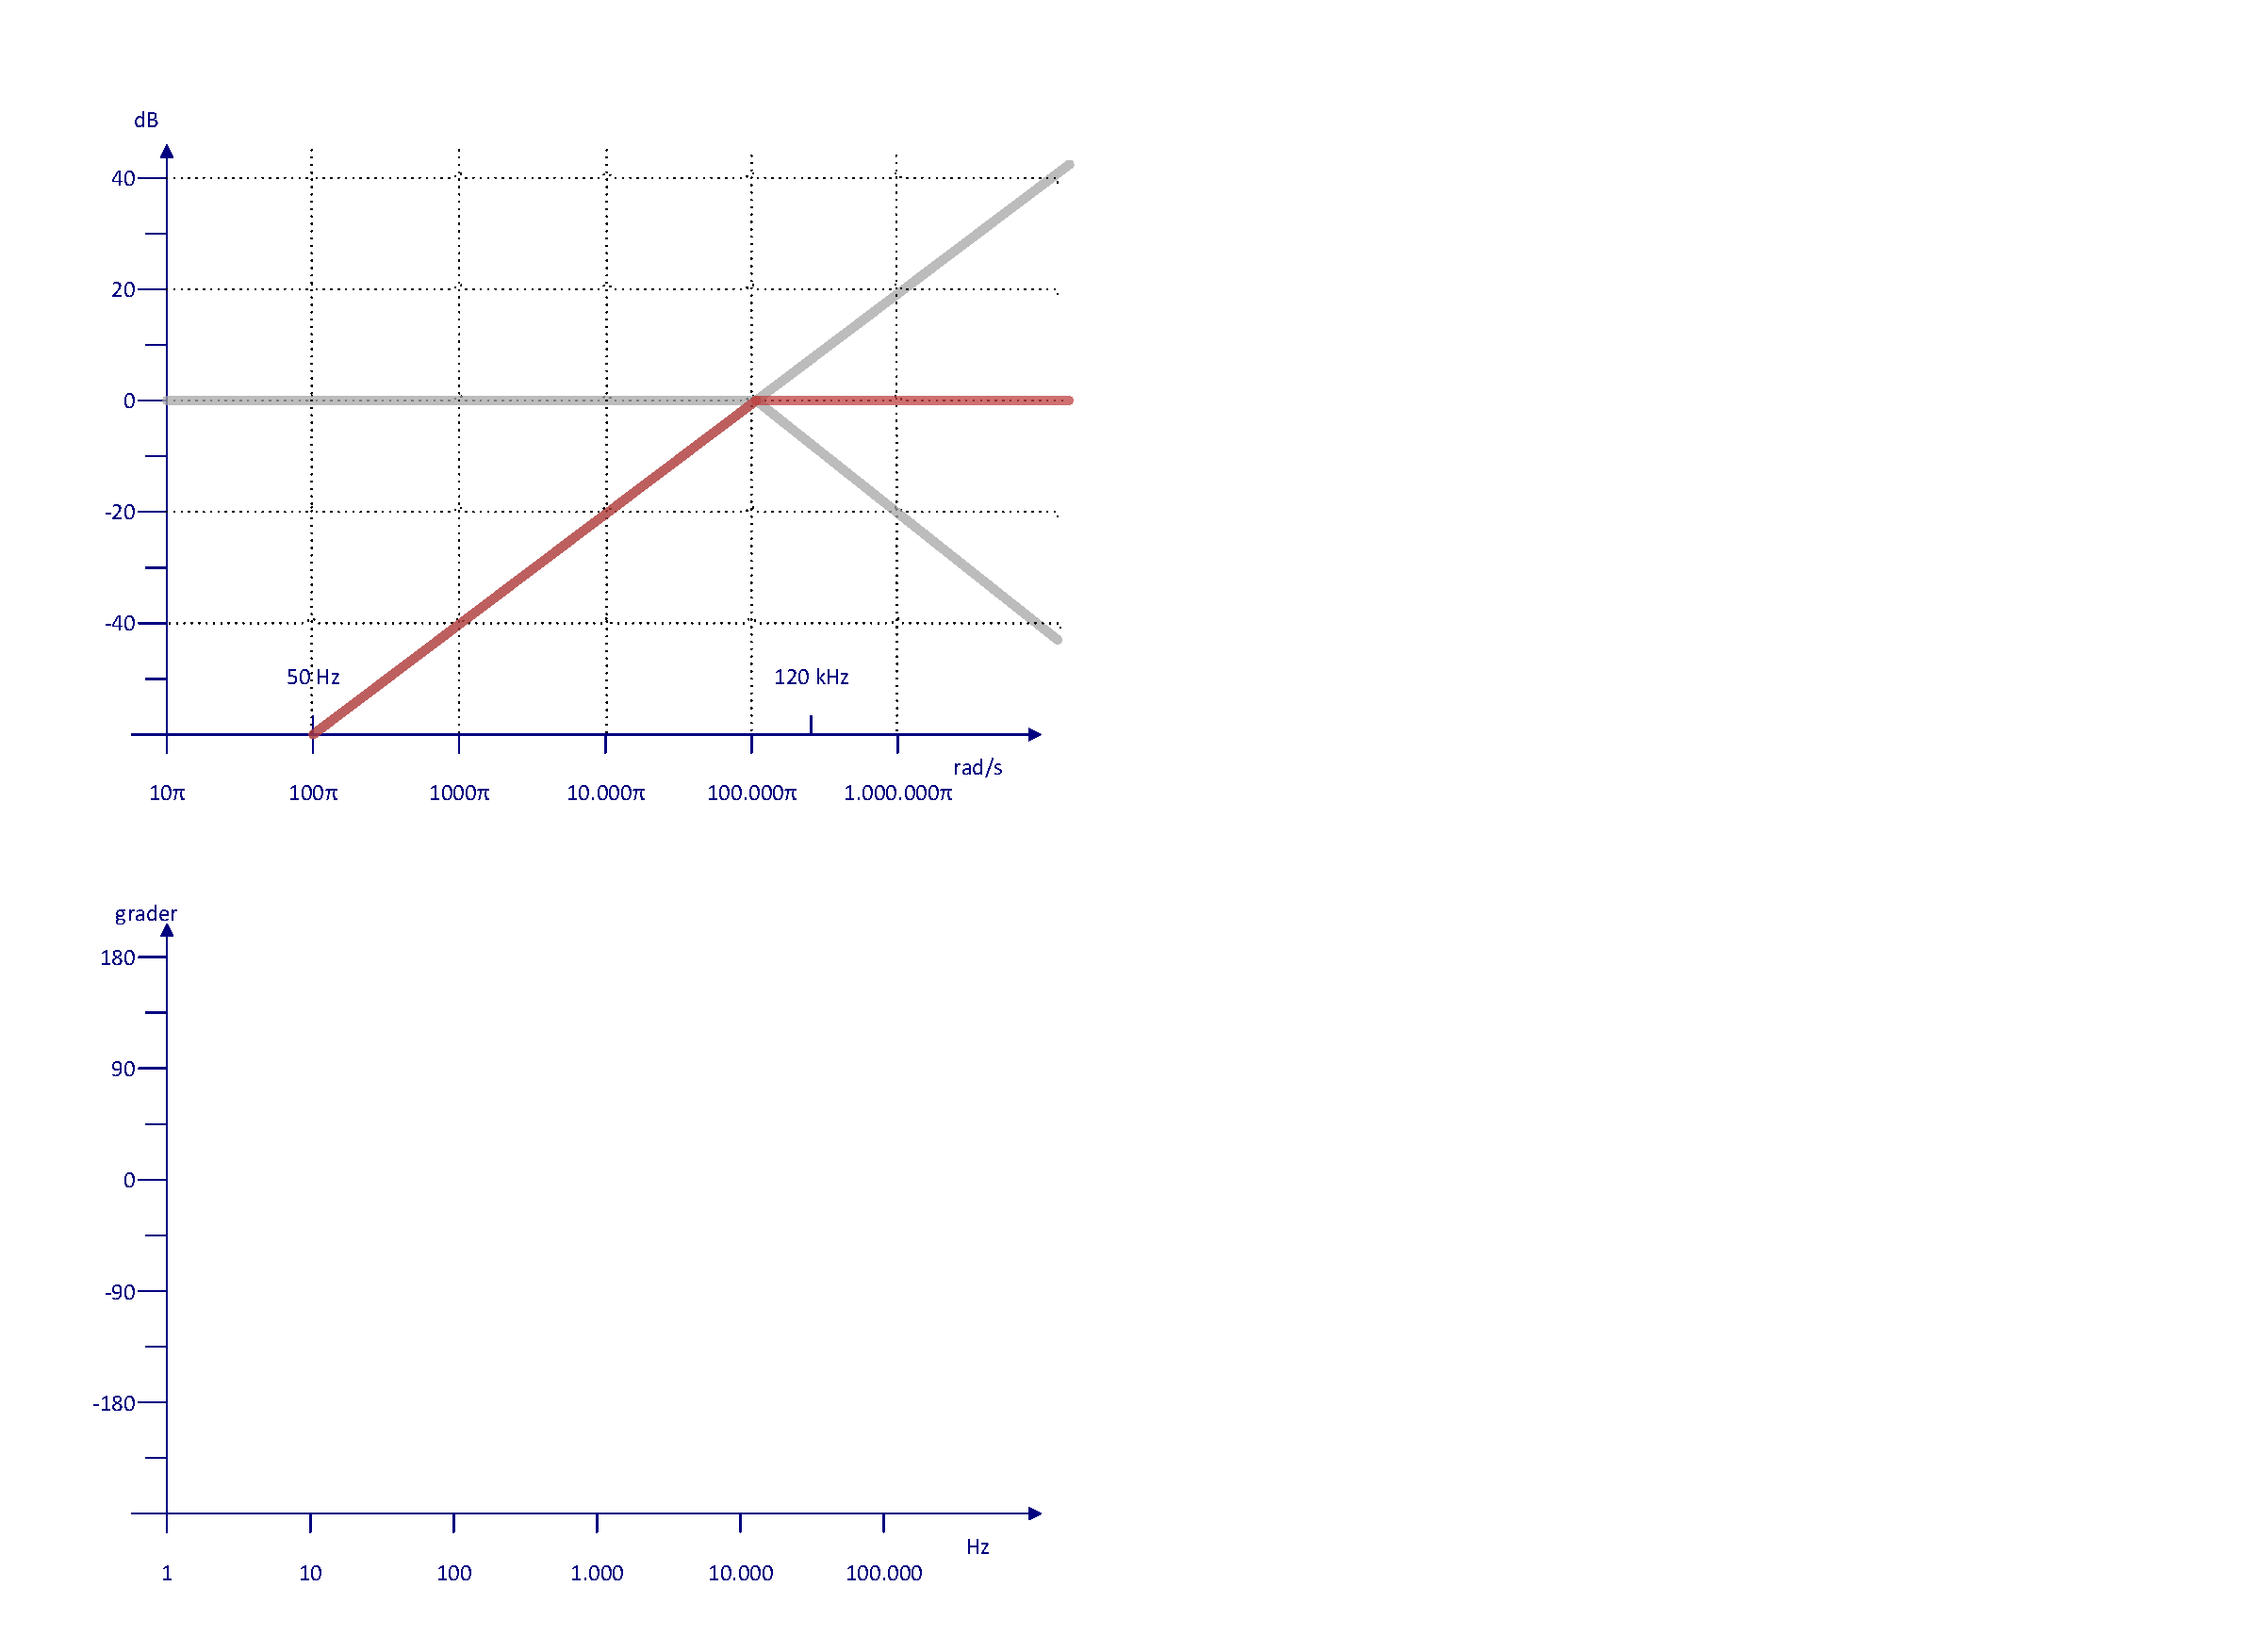
\includegraphics[scale=0.5, trim=50 420 560 50, clip=true]{../HardwareDesign/Diagrammer/BodePlotHPF.pdf}
	\caption{Bodeplot med asymptotiske linjer for højpasfilter}
	\label{fig:BodeHPF}
\end{figure}

\begin{displaymath}
T_{v}(s)\approx 
\dfrac{100\cdot 10^{3}\pi rad/s}{100\cdot 10^{3}\pi rad/s +s} \cdot \dfrac{s}{100\cdot 10^{3}\pi rad/s}
\end{displaymath}

For at bestemme komponentværdierne, fastsættes vores kondensator til $C_{6} = 1nF$. Overføringsfunktionen er omskrevet, så den består af standardled, og man kan derfor fastslå følgende:

\begin{displaymath}
\omega_{c_{2}} = \dfrac{1}{R_{6} \cdot C_{6}} \Leftrightarrow
R_{6} = \dfrac{1}{\omega_{c_{2}} \cdot C_{6}} = \dfrac{1}{100\cdot 10^{3}\pi rad/s \cdot 1\cdot 10^{-9}F} = 3183 \Omega \approx 3.3k \Omega
\end{displaymath}

Der laves et bodeplot med asymptotiske linjer, Figur \ref{fig:BodeHPF}, for at se hvordan højpasfilteret vil dæmpe/forstærke forskellige frekvenser.

\section{Receiver}

\subsection{Lysmodul (Morten)}

\begin{figure}[h]
	\centering
	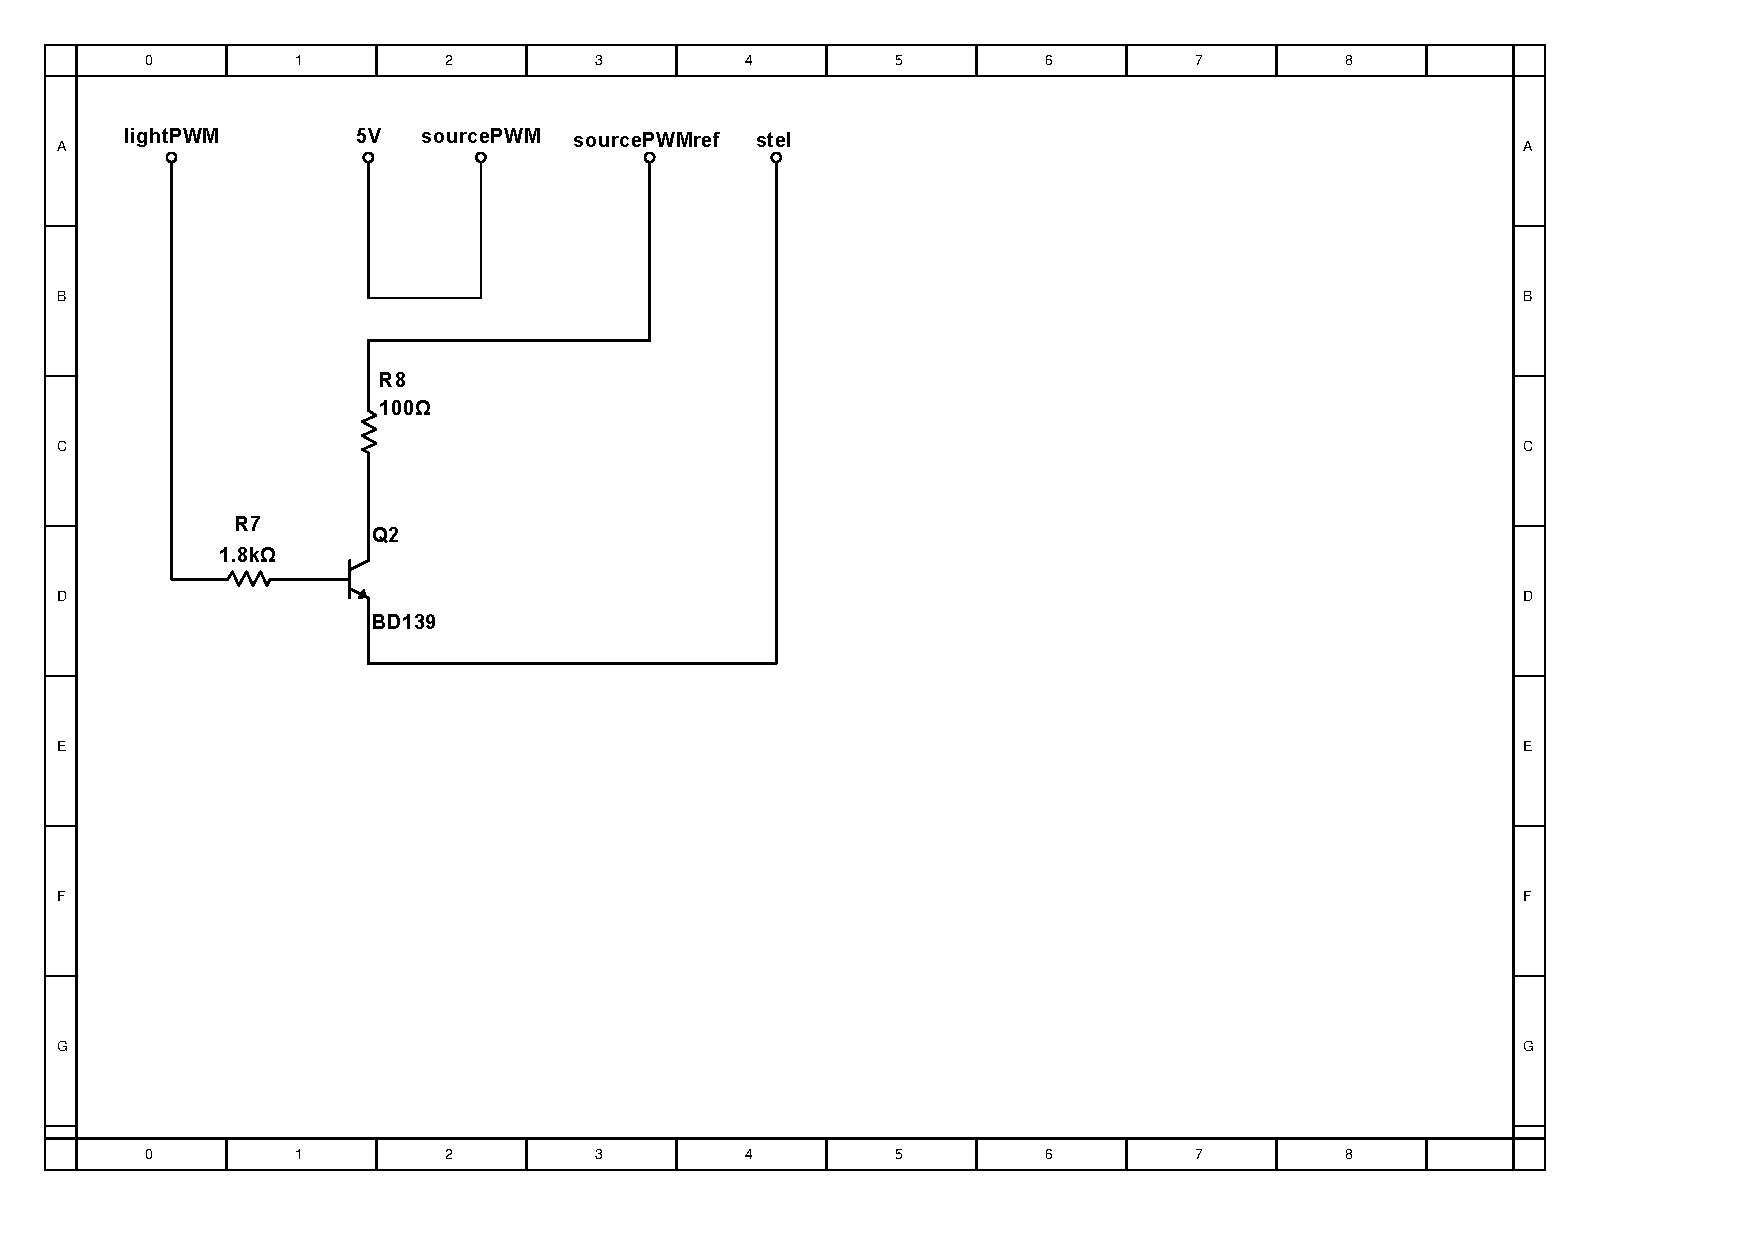
\includegraphics[scale=0.8, trim=50 250 440 60, clip=true]{../HardwareDesign/Diagrammer/Lysmodul.pdf}
	\caption{Lysmodul}
	\label{fig:Lysmodul-kredslob}
\end{figure}

Transistoren $(BD139)$\cite{lib:BD139}, $Q_{2}$, er i mætning, og styrer derved PWM-signalet til lampen vha. PWM-signalet fra STK500. På den måde undgås det, at der trækkes strøm fra STK500 til lampen, og det giver mulighed for dæmpning af lysstyrken.

$R_{8}$ beregnes udfra strøm gennem lampen og spændingsfaldet over denne. 

Som lampe anvendes en Kingbright 5mm gul diode $(L-53 YD)$\cite{lib:LED}, som jf. databladet har et typisk spændingsfald på $2.1V$ og en anbefalet middelstrøm på $30mA$.

\begin{displaymath}
R_{8} = \dfrac{5V-V_{diode}}{I_{diode}} = \dfrac{5V-2.1V}{0.03A} = 97\Omega \approx 100\Omega
\end{displaymath}

\begin{displaymath}
R_{7}\leq \beta \cdot R_{8} = 20 \cdot 100\Omega = 2000\Omega \approx 1.8k\Omega
\end{displaymath}

\subsection{Carrier Detector (Morten, Henrik og Lasse)}
Carrier detectoren kan deles op i 2 overordnede dele; et båndpasfilter og en envelope detector. Efter envelope detectoren er der desuden en operationsforstærker. Denne sætter udgangen til $5V$, når envelope detectoren udsender en spænding, der er højere end referencespændingen på operationsforstærkerens inverterende indgangsben, og $-5V$ når det er lavere. For at undgå negativ spænding på \textit{bitstream} signalet, er der koblet en diode på udgangen af operationsforstærkeren.

Båndpasfilteret består hhv. af et højpasfilter $(C_{7}$ og $R_{9})$, en ikke-inverterende opAmp uden forstærkning $(U_{3})$ og et lavpasfilter $(R_{10}$ og $C_{8})$.
\begin{figure}[h]
	\centering
	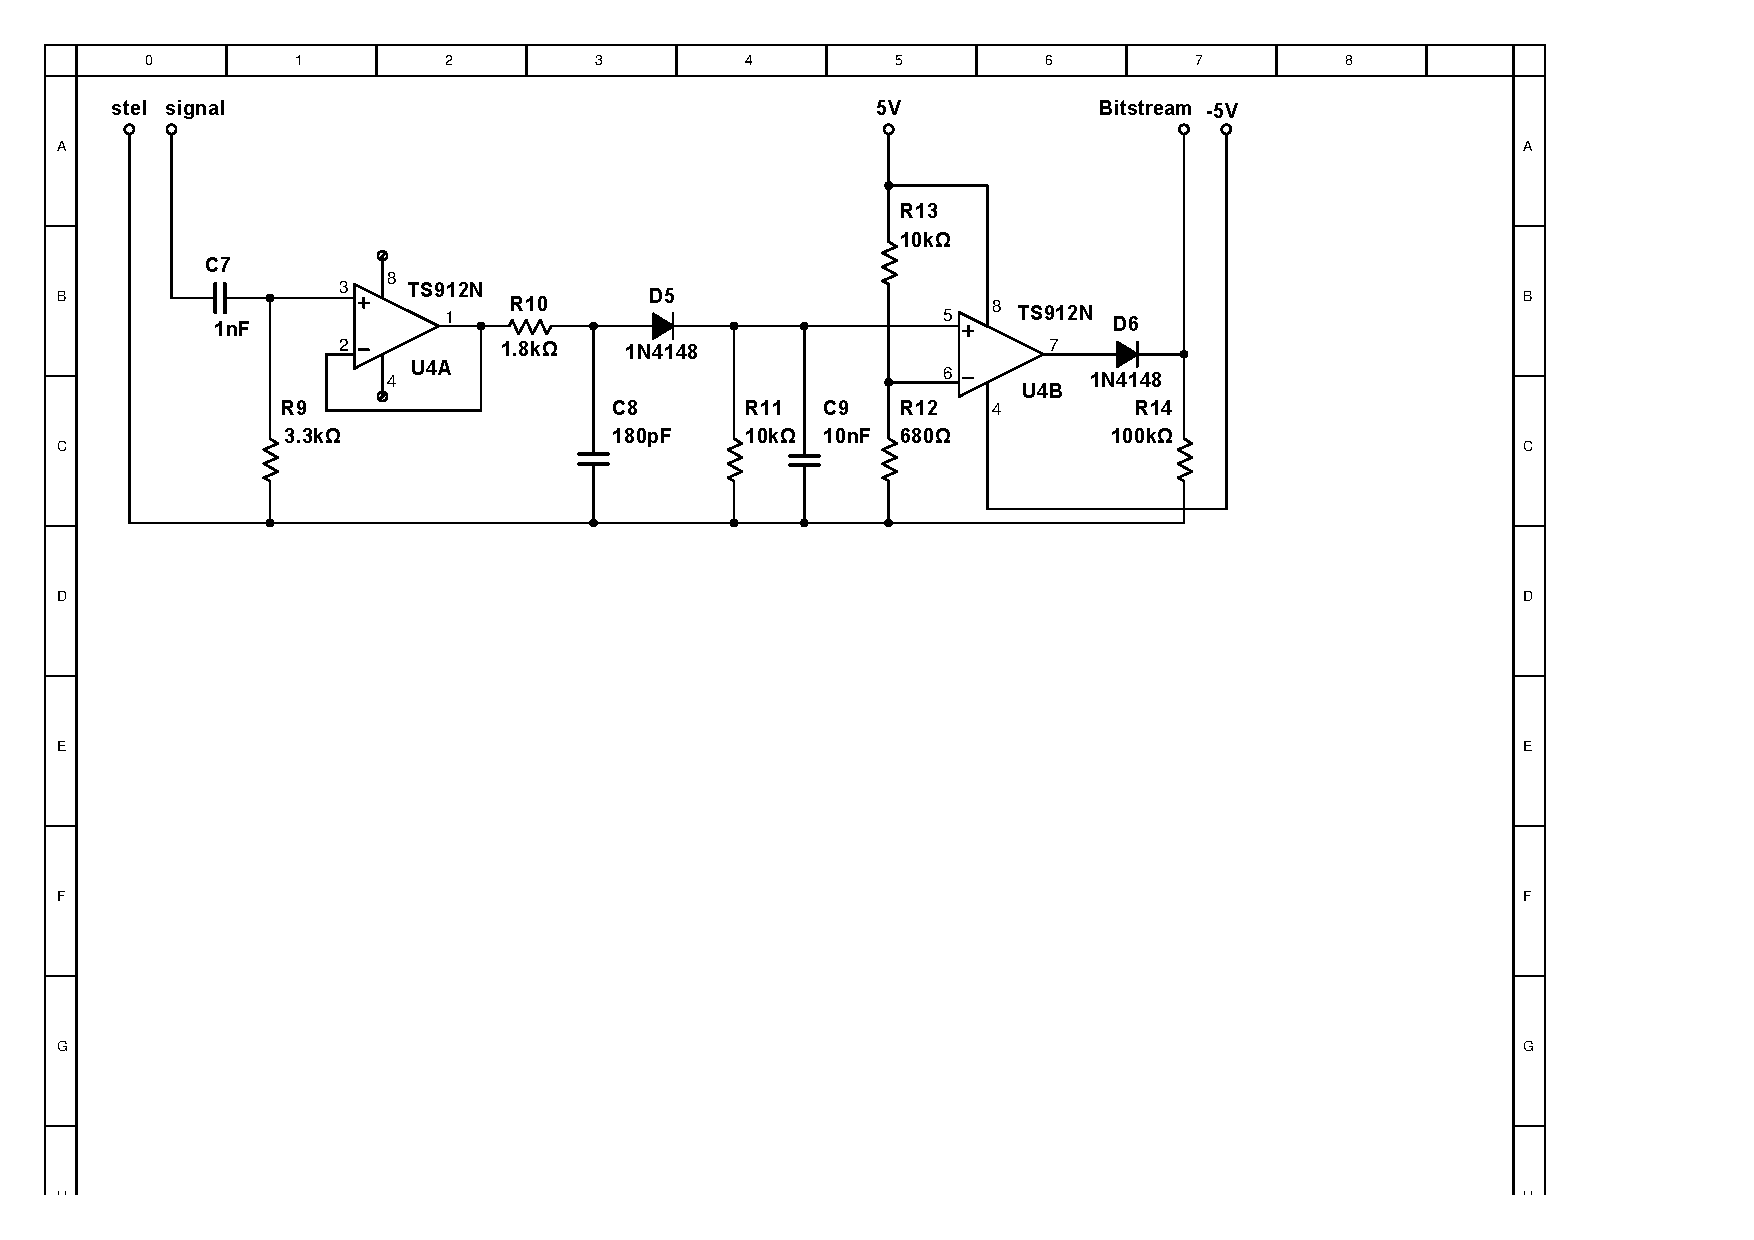
\includegraphics[scale=0.75, trim=40 340 240 40, clip=true]{../HardwareDesign/Diagrammer/CarrierDetector.pdf}
	\caption{Carrier detector}
	\label{fig:CarDetek}
\end{figure}

\subsubsection{Båndpasfilter}

For at isolere $120kHz$ signalet, benyttes et båndpasfilter. Filteret skal lade $120kHz$ passere, og frasorterer alt andet, herunder $18VAC$-$50Hz$ nettet.

Det ønskes at filteret får følgende knækfrekvenser:

\begin{displaymath}
\omega_{c_{2}} = 2 \pi \cdot 50 \cdot 10^3 Hz = 100\pi \cdot 10^{3} rad/s
\end{displaymath}
\begin{displaymath}
\omega_{c_{3}} = 2 \pi \cdot 500 \cdot 10^3 Hz = 1\pi \cdot 10^{6} rad/s
\end{displaymath}

Da kaskadereglen skal være opfyldt, indsættes et forstærkningsled med en forstærkning på $1$.

For båndpasfilteret på Figur \ref{fig:CarDetek}, opstilles følgende overføringsfunktion:

\begin{displaymath}
T_{v}(s)\approx \underbrace{\dfrac{R_{9}}{\tfrac{1}{C_{7}\cdot s}+R_{9}}}_\text{Højpas} \cdot
\underbrace{1}_\text{Gain} \cdot
\underbrace{\dfrac{ \tfrac{ 1 }{C_{8}\cdot s}}{ \tfrac{ 1 }{C_{8}\cdot s }+ R_{10}}}_\text{Lavpas}
\end{displaymath}

Overføringsfunktionen består af tre dele; et højpasfilter, en forstærkning og et lavpasfilter. Det kan ses at højpasfilteret er det samme som beskrevet i transmitter-afsnittet, og at knækfrekvensen for disse er ens.

\begin{displaymath}
C_{7} = 1nF
\end{displaymath}

\begin{displaymath}
R_{9} = \dfrac{1}{\omega_{c_{2}} \cdot C_{7}} = \dfrac{1}{100\cdot 10^{3}\pi rad/s \cdot 1\cdot 10^{-9}F} = 3183 \Omega \approx 3.3k\Omega
\end{displaymath}

Lavpasfiltrets overføringsfunktion omregnes til standard form.

\begin{displaymath}
T_{lavpas}(s)\approx \dfrac{ \tfrac{ 1 }{C_{8}\cdot s}}{ \tfrac{ 1 }{C_{8}\cdot s }+ R_{10}} = 
\dfrac{ \tfrac{ 1 }{ R_{10} \cdot C_{8}} }{ \tfrac{ 1 }{ R_{10} \cdot C_{8}} +s }
\end{displaymath}

Da lavpasfilteret er på standardform, vides det at:

\begin{displaymath}
T_{v}(s)\approx \dfrac{ \tfrac{ 1 }{ R_{10} \cdot C_{8}} }{ \tfrac{ 1 }{ R_{10} \cdot C_{8}} +s }=
\dfrac{\omega_{c_{3}}}{\omega_{c_{3}}+s}
\end{displaymath}

Kondensatoren fastsættes til $C_{8}=180pF$

\begin{displaymath}
\omega_{c_{3}} = \dfrac{ 1 }{ R_{10} \cdot C_{8}} \Rightarrow 
R_{10}=\dfrac{1}{\omega_{c_{3}} \cdot C_{8}}=
\dfrac{1}{\pi \cdot 10^{6} rad/s \cdot 180 \cdot 10^{-12}F}=1768\Omega \approx 1.8k\Omega
\end{displaymath}

Der opstilles et bodeplot med asymptotiske linjer for båndpasfilteret, Figur \ref{fig:BodePlotBPF}. 

\begin{figure}[h]
	\centering
	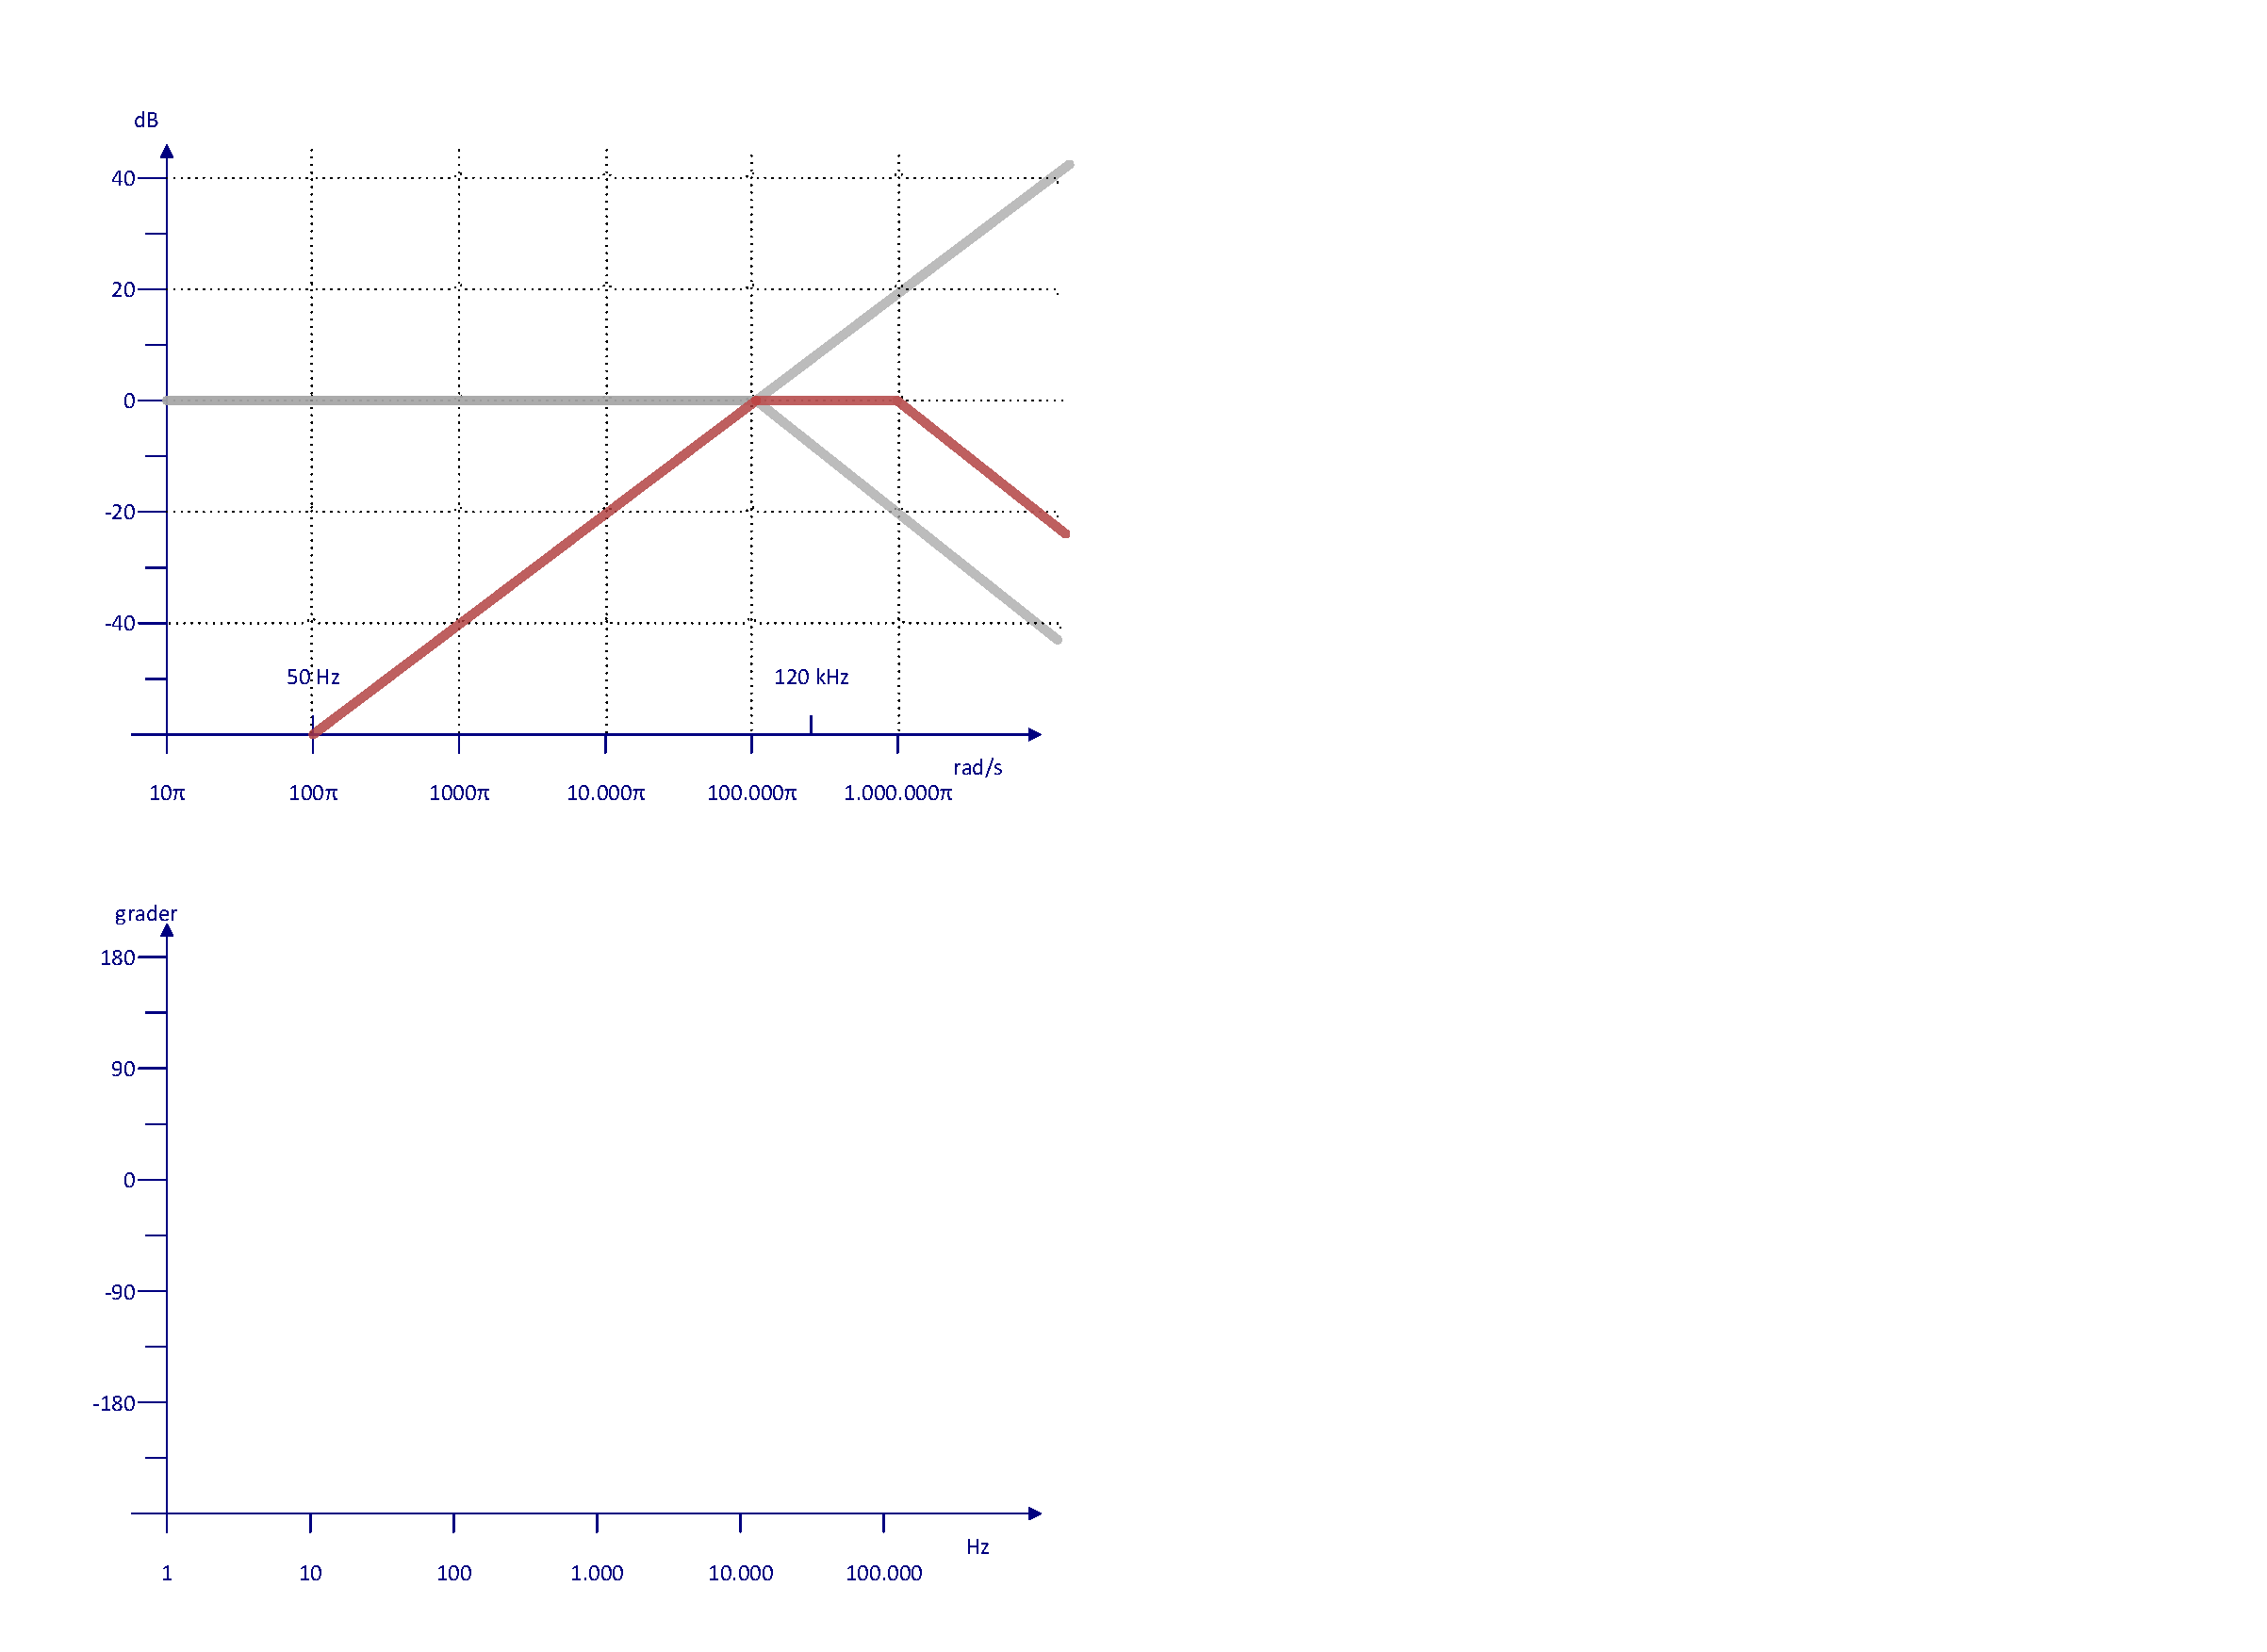
\includegraphics[scale=0.5, trim=50 430 590 50, clip=true]{../HardwareDesign/Diagrammer/BodePlotBPF.pdf}
	\caption{Bodeplot med assymptotiske linjer for båndpasfilter}
	\label{fig:BodePlotBPF}
\end{figure}

\subsubsection{Envelope Detector}
For at fortolke 120kHz signalet til et logisk signal, der går HIGH når 120kHz signalet er til stede og LOW når det ikke er til stede, er der tilkoblet en envelope detector efter båndpasfilteret.

Envelope detectoren består af modstanden $R_{11}$, kondensatoren $C_{9}$ samt dioden $D_{5}$. Dioden lader kun positive spændinger passere. Dette bevirker at i tilfælde af negativ spændinger før dioden, aflades kondensatoren i envelope detectoren ikke hurtigere end ved $0V$.

Hvert peak af inputtet vil oplade kondensatoren, der sørger for, at spændingen i punktet mellem dioden og kondensatoren holdes nær peakværdien. Modstanden i parallel med kondensatoren vil gradvist aflade kondensatoren. For at kondensatoren ikke aflades så hurtigt at spændingen falder til under den ønskede værdi imellem peaks fra 120kHz signalet, skal følgende forudsætning være opfyldt:

\begin{displaymath}
T \ll \tau
\end{displaymath}

Hvor $\tau$ er forholdet mellem modstand og kondensator ($\tau = R_{11} \cdot C_{9}$). $T$ er en tidsperiode ($T = f^{-1}$).

Sættes der værdier ind, findes tidsperioden til:

\begin{displaymath}
T = \tfrac{1}{120kHz} \approx 8.3 \mu s 
\end{displaymath}

Herefter bestemmes $\tau$ til at være $100 \mu s$. Derved aflades kondensatoren langsomt nok til, at den ikke kommer under den ønskede tærskel, men ikke for langsomt i forhold til næste nul-gennemgang på $18VAC$-$50Hz$ nettet.

Modstanden sættes til $10k\Omega$, dermed bliver kondensatorens størrelse:

\begin{displaymath}
C_{9} = \tfrac{\tau}{R_{11}} = \tfrac{100\cdot 10^{-6}s}{10 \cdot 10^{3}\Omega} = 10 \cdot 10^{-9}F = 10 nF
\end{displaymath}

\subsubsection{Komparator}
Ovenstående del af carrier detectoren er testet på fumlebræt ved brug af carrier generatoren. Ved testen måltes $480-600mV$ på envelope detectoren, ved detektion af 120kHz signal, og ca. $0V$ uden detektion af signal. Derfor er der lavet en spændingsdeler som giver OP-ampens\cite{lib:TS912} inverterende indgang en reference på:

\begin{displaymath}
V_{ref}= 5V \cdot \left(\dfrac{R_{12}}{R_{12}+R_{13}}\right)=5V \cdot \left(\dfrac{680\Omega}{680\Omega + 10 \cdot 10^{3}\Omega}\right)=318mV
\end{displaymath}

Dette betyder at der på OP-ampens udgang er $+5V$ hvis spændingen på envelope detectoren er over referencen, og $-5V$ hvis den er under refenrecen. For at undgå negativ spænding på \textit{bitstream} signalet, er der plaseret en diode ($D_{6}$), som forhindrer dette. Der er et mindre spændingfald over dioden, men dette har ingen betydning. Derudover er der forbundet en pull-down modstand ($R_{14}$) efter dioden for at sikre at \textit{bitstream} ligger stabilt på $0V$, når operationsforstærkeren leverer negativ spænding.

\clearpage